
\documentclass[border={0pt 0pt 0pt 0pt}]{standalone}
\usepackage{tikz-cd,tikz-3dplot} 
\usetikzlibrary{calc,intersections,through,backgrounds,decorations.pathmorphing, decorations.shapes,decorations.markings,patterns}
%include other needed packages here   
\begin{document}
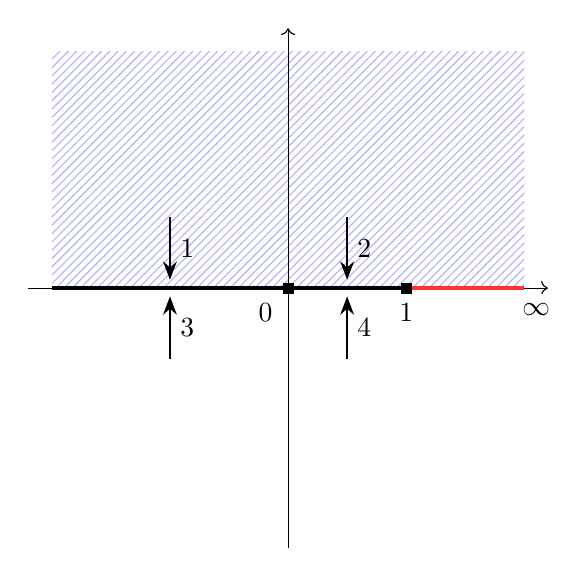
\begin{tikzpicture}[scale=3]

\fill[pattern=north east lines, pattern color=blue!30!white] (-1,0) rectangle (1,1);

\foreach \y/\ytext in {-0.5/3,0.25/4}
\draw[-{Stealth[]},thick] (\y cm,-0.3cm) to node[anchor=west] {$\ytext$} (\y cm,-1pt);
\foreach \x/\xtext in {-0.5/1,0.25/2}
\draw[-{Stealth[]},thick] (\x cm,0.3cm) to node[anchor=west] {$\xtext$} (\x cm,1pt);


\draw[->] (-1.1,0) -- (1.1,0);
\draw[->] (0,-1.1) -- (0,1.1);

\draw (-0.7pt,-0.7pt)  node[anchor=north east,fill=white] {0};
\draw (0.5,-0.7pt)  node[anchor=north,fill=white] {1};
\draw (1.05,-0.7pt)  node[anchor=north,fill=white] {$\infty$};
\draw[red!80!white,very thick] (0.5,0) -- (1,0);
\draw[very thick] (0.5,0) -- (-1,0);
\node [fill=black,inner sep=2pt] at (0,0) {};
\node [fill=black,inner sep=2pt] at (0.5,0) {};
\end{tikzpicture}
\end{document}